%!TEX root = ../TechnischerEntwurf.tex

\chapter{Einleitung}
Dieses Dokument dient dazu, einen tiefer gehenden Überblick über den internen Ablauf der zu entwickelnden Software zu bieten. Es werden zuerst die wichtigsten Funktionen einzeln beschrieben, wobei Sequenzdiagramme zu Hilfe genommen werden. Danach wird der Aufbau der Komponenten beschrieben, sowie deren Verteilung gezeigt und am Ende die Datenverwaltung näher beleuchtet. \\
Ziel ist es, dass ein Entwickler nach dem Lesen dieses Dokuments die Software nachentwickeln könnte.

\begin{figure}[h]
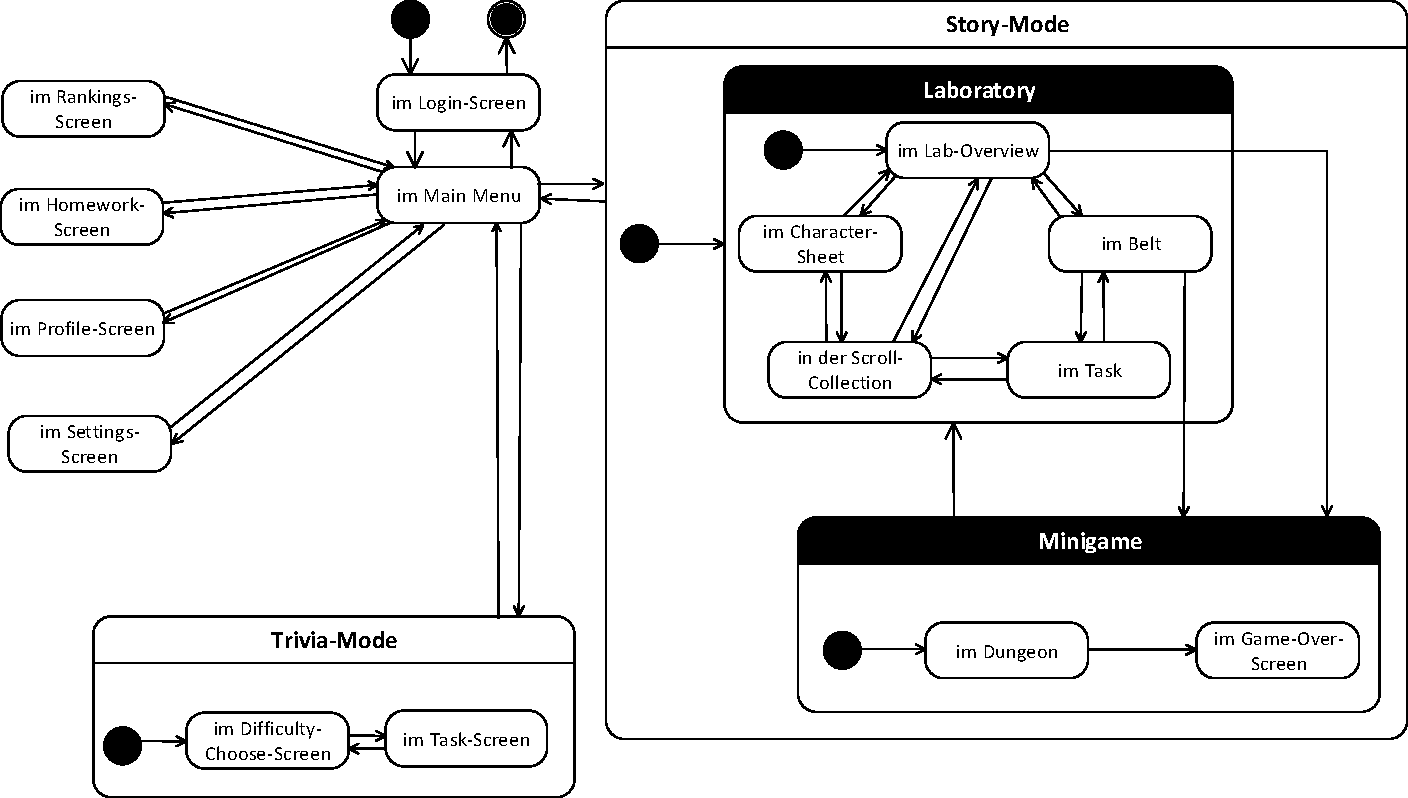
\includegraphics[width=1.0\textwidth]{figures/statechart_game.pdf}
\caption{Zustandsdiagramm zum oberflächlichen Spielablauf}
\label{state_game}
\end{figure}


Um eine Verständnisgrundlage zu schaffen ist in Abbildung 1.1 die allgemeine Men\"uf\"uhrung in einem Zustandsdiadramm dargestellt. 


Nach dem Einloggen gelangt man in das Main Menu. Von dort aus gelangt man in die drei Spielmodi (Story, Trivia, Homework), die Einstellungen, das Profil und in die Ranglisten.

Der Story Mode hat wiederum eine eigene Übersicht, Laboratory genannt. Von hier aus kann der User sich seine aktuellen Playerstatistiken im Charakter Sheet ansehen, kann sich in der Scrollcollection um die Herstellung von Potions und Enchantments k\"ummern, diese danach in seinen Belt einf\"ugen um sich im Anschluss dem Minispiel zu widmen. Im Minispiel werden dem User verschiedene Hindernisse vorgesetzt, die es zu überwinden gilt. Scheitert der User, so gelangt er in den Game Over Screen, in dem ihm angezeigt wird wie viele Lofi-Coins (die Spiel-Währung) und welche Scrolls er in dieser Runde eingesammelt hat. Nach Bestätigung befindet sich der User zurück im Laboratory.

Der Trivia-Mode stellt einen SQL-Trainer dar. Entscheidet der User sich dafür diesen zu verwenden, gelangt er in einen Screen, in dem er sich für einen Schwierigkeitsgrad entscheiden muss. Hat der User dies getan, erhält er eine, dem ausgewählten Schwierigkeitsgrad entsprechende, Aufgabe und kann diese lösen.

Der Homework-Mode funktioniert auf die gleiche Weise wie der Trivia-Mode, lediglich die Auswahl des Schwierigkeitsgrads entf\"allt in diesem Fall.
Die Funktion soll den Hausaufgaben-Ablauf der Vorlesung RDB1 unterstützen.

In den Rankings werden die Spieler nach verschiedenen Kriterien in Ranglisten sortiert. Darüber ist es auch möglich, durch die Eingabe des Benutzernamens, nach anderen Spielern zu suchen und sich deren Profil anzeigen zu lassen.
Das eigene Profil ist über das Main Menu zu erreichen und einsehbar. Selbiges gilt für die Spieleinstellungen.  



\section{Projektdetails}

Die Anzahl an Lofi-Coins, sowie die Anzahl an Scrolls, die der User pro Tag einsammeln kann, werden beschr\"ankt.
Dies soll verhindern, dass der User hauptsächlich oder ausschließlich das Minispiel spielt, was dem Zweck der Anwendung, nämlich dem Üben von SQL entgegenwirkt. Auf der anderen Seite soll so der Spieler zum Wiederkommen animiert werden.

Des Weiteren wurde im Pflichtenheft erwähnt, dass Spieler sich durch Aufgabenerstellung ins Spiel mit einbringen können. Um dabei jedoch eine gewisse Qualität gewährleisten zu k\"onnen, wird es nur beförderten Nutzern möglich sein, eigene Aufgaben zu erstellen. Wie ein User befördert wird, wird über die Spielzeit oder über Leistungen im Spiel geregelt.  




%\chapter{Einleitung}

%Hier erfolgt eine kurze Darstellung von Aufbau und Ziel dieses Dokuments.

%Hier ist die Arbeitsweise des Systems anhand von Aktivitätsdiagrammen 
%und/oder Statecharts darzustellen und kurz verbal beschreiben.



%Beispiele:
%\begin{itemize}
%\item Bei einem Spiel könnte der Ablauf des Spiels als Aktivitätsdiagramm dargestellt werden.
%\item In einen Web-System könnten die vom Nutzer sichtbaren Seiten als Zustände im Statechart modelliert werden.
%\end{itemize}

%\begin{figure}[ht]
%\centering
%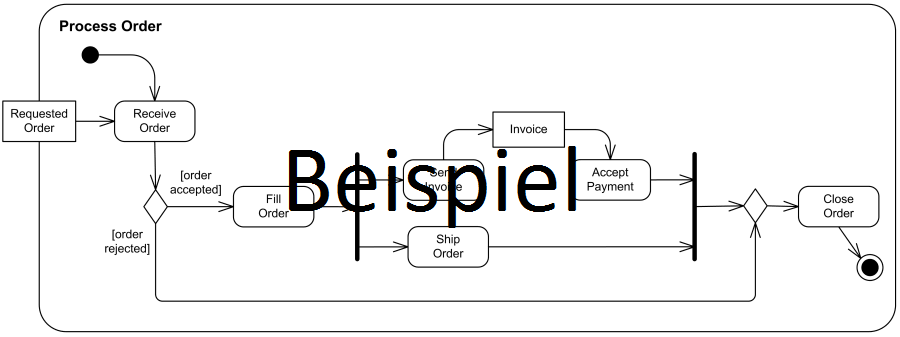
\includegraphics[width=0.7\textwidth]{figures/activity}
%\caption{Ein beispielhaftes Aktivitätsdiagramm}
%\label{activity}
%\end{figure}

%Quelle der Abbildung \ref{activity}: http://www.uml-diagrams.org/

%\textbf{Hinweis zu den Templates:}\\
%Dieses Template enthält Hinweise und Beispiele, die selbstverständlich zu entfernen sind.
% Angaben in <...> sind mit dem entsprechendem Text zu füllen.
%Die Grafiken in diesem Dokument sind nur Beispiele und sind keine Vektorgrafiken. 

%\textbf{Aufgabe des Technischen Entwurfs:}\\
%Der Technische Entwurf dokumentiert die klassischen Entwurfsentscheidungen wie z.B. 
%die Verwendung bestimmter Bibliotheken oder Entwurfsmuster. Darüber hinaus bildet der 
%Technische Entwurf die Grundlage der Implementierung, d.h. anhand dieses Dokumentes 
%muss jeder Softwareentwickler in der Lage sein, das Produkt zu entwickeln.
% Es ist also auf Vollständigkeit der Dokumentation zu achten.\\
%\textbf{Kapitel die bereits im Fachentwurf bearbeitet wurden, müssen hier nicht erneut
% bearbeitet werden. Es sollten jedoch die Annotationen umgesetzt worden sein.
% Es sollen also Kapitel 3-5 und Kapitel 8-9 neu erarbeitet werden. Kapitel 10 soll an 
%dieses Dokument angepasst werden, wenn es notwendig ist.}

%\textbf{Dieses Kapitel kann aus dem Fachentwurf übernommen werden, 
%sollte jedoch die Bearbeitung der Annotationen beinhalten.}

%\section{Projektdetails}

%Besonders interessante oder komplizierte Sachverhalte sollen hier noch weiter vertieft werden.
% Auch hier sollen wieder Aktivitätsdiagrame und Statecharts verwendet werden.

%Beispiele:
%\begin{itemize}
%\item Bei einem Spiel könnten komplizierte Regeln dargestellt werden.
%\item In einen Web-System könnte bestimmte Workflows als Aktivitätsdiagramm dargestellt werden.
%\end{itemize}

%Es kann pro Sachverhalt ein Abschnitt hinzugefügt werden.

